% This file was created with tikzplotlib v0.10.1.
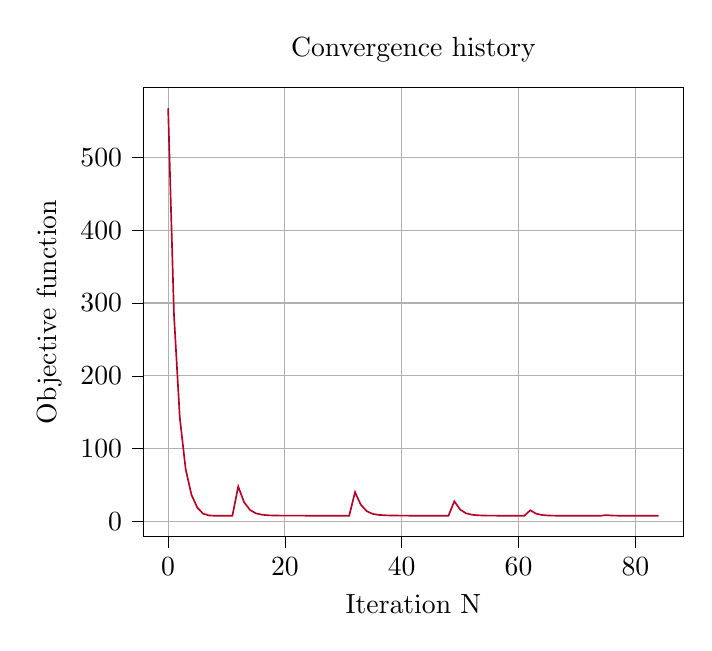
\begin{tikzpicture}

\definecolor{darkgray176}{RGB}{176,176,176}
\definecolor{firebrick180438}{RGB}{180,4,38}

\begin{axis}[
tick align=outside,
tick pos=left,
title={Convergence history},
x grid style={darkgray176},
xlabel={Iteration N},
xmajorgrids,
xmin=-4.2, xmax=88.2,
xtick style={color=black},
xtick={-20,0,20,40,60,80,100},
xticklabels={
  \(\displaystyle {\ensuremath{-}20}\),
  \(\displaystyle {0}\),
  \(\displaystyle {20}\),
  \(\displaystyle {40}\),
  \(\displaystyle {60}\),
  \(\displaystyle {80}\),
  \(\displaystyle {100}\)
},
y grid style={darkgray176},
ylabel={Objective function},
ymajorgrids,
ymin=-20.4660621481687, ymax=595.740936825826,
ytick style={color=black},
ytick={-100,0,100,200,300,400,500,600},
yticklabels={
  \(\displaystyle {\ensuremath{-}100}\),
  \(\displaystyle {0}\),
  \(\displaystyle {100}\),
  \(\displaystyle {200}\),
  \(\displaystyle {300}\),
  \(\displaystyle {400}\),
  \(\displaystyle {500}\),
  \(\displaystyle {600}\)
}
]
\addplot [semithick, firebrick180438]
table {%
0 567.731527781554
1 284.156907647447
2 142.418543655861
3 71.6279206294987
4 36.2985177279511
5 18.7364030357227
6 10.4627874735361
7 8.07531444671416
8 7.58423156776642
9 7.58311226979672
10 7.58308569635584
11 7.58308538976737
12 47.8616750325681
13 26.3409862687484
14 15.722804288627
15 11.0079844770942
16 9.11964475121681
17 8.3030777972484
18 7.984101656675
19 7.85622433589438
20 7.8056164571903
21 7.78417727486958
22 7.77157837794479
23 7.75729301096695
24 7.71422375162625
25 7.68868323243131
26 7.67730747688736
27 7.6716866708577
28 7.66890970311566
29 7.66752899137718
30 7.66686835539854
31 7.66658178891932
32 40.1213056391837
33 22.6153560484249
34 13.9435296562586
35 10.2323366558581
36 8.84417509644219
37 8.29778927774505
38 8.0281482650998
39 7.88700348052655
40 7.82128638769147
41 7.76701818558912
42 7.63647600286573
43 7.58564233031811
44 7.57215621038791
45 7.56980834396136
46 7.56939134519209
47 7.5692168475264
48 7.56912749545959
49 27.6053592255639
50 16.0929053064439
51 11.0198025432695
52 9.07048319421829
53 8.26659535315516
54 7.93309514287235
55 7.79734455460412
56 7.74322856085269
57 7.71949202337723
58 7.70825147530375
59 7.70297290093864
60 7.70075806959413
61 7.70002186505958
62 15.1669301659655
63 10.4829794160759
64 8.68463983249225
65 8.02333398056093
66 7.76533920813542
67 7.65973043898608
68 7.60889646001775
69 7.58554849475508
70 7.57502427949564
71 7.56974127902061
72 7.56759101669718
73 7.56690639538894
74 7.56673367666218
75 8.53812275207694
76 7.91265977513176
77 7.72236993991236
78 7.64117003667948
79 7.60227349399293
80 7.57261867635168
81 7.55573012730278
82 7.54786810854061
83 7.54464514138901
84 7.54334689610382
};
\end{axis}

\end{tikzpicture}
